%%%%%%%%%%%%%%%%%%%%%%%%%%%%%%%%%%%%%%%%%
% Wenneker Assignment
% LaTeX Template
% Version 2.0 (12/1/2019)
%
% This template originates from:
% http://www.LaTeXTemplates.com
%
% Authors:
% Vel (vel@LaTeXTemplates.com)
%
% License:
% CC BY-NC-SA 3.0 (http://creativecommons.org/licenses/by-nc-sa/3.0/)
% 
%%%%%%%%%%%%%%%%%%%%%%%%%%%%%%%%%%%%%%%%%

%----------------------------------------------------------------------------------------
%	PACKAGES AND OTHER DOCUMENT CONFIGURATIONS
%----------------------------------------------------------------------------------------

\documentclass[11pt]{scrartcl} % Font size
\input{structure.tex} % Include the file specifying the document structure and custom commands

%----------------------------------------------------------------------------------------
%	TITLE SECTION
%----------------------------------------------------------------------------------------

\title{	
	\normalfont\normalsize
	\rule{\linewidth}{0.5pt}\\ % Thin top horizontal rule
	\vspace{10pt} % Whitespace
	{\huge Rozwiązywanie Sudoku przy pomocy algorytmu genetycznego oraz algorytmu ACO}\\ % The assignment title
	\vspace{12pt} % Whitespace
	\rule{\linewidth}{2pt}\\ % Thick bottom horizontal rule
}

\author{\LARGE Bartosz Cywiński, Łukasz Staniszewski} % Your name

\date{} % Today's date (\today) or a custom date

\begin{document}

\maketitle % Print the title
%----------------------------------------------------------------------------------------
%	FIGURE EXAMPLE
%----------------------------------------------------------------------------------------

\section{Opis problemu}
Podstawowa wersja Sudoku składa się z dwuwymiarowej planszy 9x9, podzielonej na 9 pól 3x3. Planszę Sudoku da się jednak rozszerzać do większych rozmiarów. Plansza na początku gry częściowo uzupełniona jest liczbami. Początkowy rozkład liczb ma duże znaczenie dla dalszego przebiegu gry – jest on jedynym czynnikiem decydującym o trudności danej wersji Sudoku. Celem rozwiązania łamigłówki jest takie ułożenie cyfr od 1 do 9, aby w każdym rzędzie, każdej kolumnie i każdym polu 3x3 każda cyfra występowała dokładnie jeden raz. Zostało udowodnione, że problem rozwiązania Sudoku jest problemem NP-trudnym, dlatego też jest on dobrym testem efektywności algorytmów.

%------------------------------------------------
\section{Opis rozwiązania przy pomocy algorytmu ACO}

\subsection{Pseudokod i opis algorytmu}
\begin{algorithm}
\caption{Algorytm ACS do rozwiązywania Sudoku}\label{alg:cap}
\begin{algorithmic}[1]
\State \texttt{wczytaj planszę Sudoku}
\For{\texttt{komórka z wybraną wartością}}
	\State \texttt{aktualizuj możliwe do przyjęcia wartości przez sąsiadów tej komórki}
\EndFor
\State \texttt{zainicjuj tablicę feromonów}
\While {\texttt{!stop}}
	\State \texttt{daj każdej mrówce kopię planszy Sudoku}
	\For{\texttt{liczba komórek}}
		\For{\texttt{liczba mrówek}}
			\If{\texttt{komórka nie ma wybranej wartości}}	
				\State \texttt{wybierz wartość dla komórki}
				\State \texttt{aktualizuj ograniczenia}
				\State \texttt{aktualizuj lokalny feromon}
			\EndIf
		\EndFor
	\EndFor
	\State \texttt{znajdź najlepszą mrówkę}
	\State \texttt{aktualizuj tablicę feromonów}
	\State \texttt{parowanie najlepszej wartości}
\EndWhile

\end{algorithmic}
\end{algorithm}

W zaproponowanym rozwiązaniu użyty został algorytm Ant Colony System (ACS), będący ulepszoną wersją klasycznego algorytmu Ant System (AS). Jego cechą charakterystyczną jest zastosowanie lokal\-nych aktualizacji feromonów przez każdą mrówkę oraz to, że tylko najlepsza mrówka aktualizuje globalne wartości tablicy feromonów. Ponadto po każdym wybraniu nowego elementu rozwiązania (wpisaniu cyfry w wybraną komórkę planszy) aktualizowane zostają wszystkie wartości możliwe do przyjęcia przez komórki planszy oraz spełniające zasady łamigłówki, ponieważ na skutek wybrania elementu rozwiązania mogły się one zmienić.\\


\textit{Linie 2-4:} Każda komórka o indeksie $i$ na początku algorytmu posiada taki sam zbiór możliwych wartości do przyjęcia ($\mathbb{V}_i=\{1,...,9\}$). Aktualizacje ograniczeń komórek z wybraną wartością polegają na:
\begin{itemize}
	\item Eliminacji z $\mathbb{V}_i$ wartości wybranych przez sąsiadów komórki $i$, gdzie sąsiedzi to wszystkie komór\-ki w tym samym rzędzie, tej samej kolumnie oraz tym samym polu 3x3, 
	\item Jeśli $|\mathbb{V}_i| = 1$, to przypisz wartość do komórki. 
\end{itemize}


\textit{Linia 5:} Dla Sudoku o wymiarze $d$ definiujemy dwuwymiarową globalną tablicę feromonów $\tau$, w której każdy element jest oznaczony jako $\tau_{i}^{k}$, gdzie $i$ to indeks komórki planszy $(0\leq{i}\leq{d^2-1})$, a $k$ to możliwa wartość do przyjęcia przez komórkę $(k\in{[1,d]})$. Każdy element tablicy feromonów inicjowany jest wartością $\tau_{0}=\frac{1}{c}$, gdzie $c=d^2$ jest całkowitą liczbą komórek planszy. W tablicy trzymane są wartości feromonów każdej możliwej do przyjęcia wartości w każdej komórce planszy.\\

\textit{Linie 8-10:} Zbiór $m$ mrówek buduje częściowe rozwiązanie $s^p$ ze skończonego zbioru możliwych elementów rozwiązania $\textbf{C} = \{c_{i}^{k}\}$, $i=0,...,d^2 -1,$ $k\in{[1,d]}$, gdzie $i$ to indeks komórki planszy, a $k$ to możliwa cyfra do wpisania w komórkę. Każda mrówka zaczyna od losowo wybranej komórki planszy Sudoku. Przechodzi ona po każdej możliwej komórce na planszy. Za każdym razem, kiedy mrówka natrafia na komórkę, która nie ma przypisanej wartości, podejmuje ona decyzję jaka to powinna być wartość i ją przypisuje - do $s^p$ dodawany jest element rozwiązania ze zbioru $\textbf{N}(s^p)\subseteq{\textbf{C}}$, który jest zdefiniowany jako zbiór elementów, które mogą być dodane do częściowego rozwiązania $s^p$ bez naruszenia założonych ograniczeń.\\

\textit{Linia 11:} Wybór wartości dla komórki $i$ dokonywany jest za pomocą stochastycznego mechanizmu uwzględniającego wartości w tablicy feromonów. Zdefiniujmy zbiór $\mathbb{V}_i$, jako zbiór możliwych do przyjęcia wartości przez komórkę $i$. Istnieją do wyboru dwie metody:
\begin{itemize}
	\item Selekcja zachłanna, gdzie wybieramy element ze zbioru $\mathbb{V}_i$ z najwyższą wartością w tablicy feromonów, 
	\item Selekcja ruletkowa, gdzie prawdopodobieństwa są proporcjonalne do wartości w tablicy feromonów. 
\end{itemize}
Prawdopodobieństwa wybierane są na podstawie parametru $ q_0\in{[0,1]} $. Kolejny element rozwiązania $s$ jest zatem wybierany według wzoru:
\begin{equation}
s = \begin{cases}
\argmax_{{k\in\mathbb{V}_i}}{\tau_i^k}, & \text{jeśli $q\leq{q_0}$},\\
$R$, & \text{w pozostałych przypadkach},
\end{cases}
\end{equation}
gdzie wartość $ q \in{[0,1]}$ losowana jest z rozkładem jednostajnym, natomiast $R$ jest określona jako:
\begin{equation}
p_{i}^{k} =
\dfrac{\tau_{i}^{k}}{\sum_{j\in{\mathbb{V}_i}}{\tau_i^j}}, k\in\mathbb{V}_i
\end{equation}
gdzie $p_{i}^{k}$ to prawdopodobieństwo wyboru $k$ z $\mathbb{V}_i$ na miejscu o indeksie $i$.\\

\textit{Linia 13:} Aktualizowanie lokalnego feromonu wspomaga eksplorację przestrzeni przeszukiwań. Za każdym razem kiedy wartość $s$ zostaje przypisana do komórki w planszy o indeksie $i$, aktualizacja następuje według formuły:
\begin{equation}
\tau_i^s = (1 - \varphi)\tau_i^s + \varphi\tau_0,
\end{equation}
gdzie $\varphi \in (0,1]$ to parametr rozpadu feromonu, który jest zazwyczaj mały, a $\tau_0$ jest początkową wartością feromonu.\\


Celem aktualizacji tablicy feromonów jest zwiększenie wartości feromonów związanych z dobrymi rozwiązaniami i zmniejszenie wartości związanych z gorszymi rozwiązaniami.\\

\textit{Linie 17-18:} Aby znaleźć najlepsze rozwiązanie, należy znaleźć najlepszą mrówkę w iteracji, czyli taką, która uzupełniła najwięcej komórek w planszy Sudoku w danej iteracji algorytmu. Aktualizacja tablicy feromonów następuje według wzoru:
\begin{equation}
\tau_i^s = \begin{cases}
(1-\rho)\tau_i^s+\rho\Delta\tau_i^s, & \text{jeśli najlepsze rozwiązanie w iteracji jest najlepsze globalnie},\\
\tau_i^s, & \text{w pozostałych przypadkach,}
\end{cases}
\end{equation}
gdzie $\rho \in [0,1]$ to parametr parowania feromonu, a $\Delta\tau_i^s$ można przyjąć jako:
\begin{equation}
\Delta\tau_i^s = \dfrac{c}{c-f_{best}},
\end{equation}
gdzie $f_{best}$ to liczba komórek uzupełnionych przez najlepszą mrówkę, a $c$ to całkowita liczba komórek na planszy.\\

\textit{Linia 19:} Na koniec stosowane jest parowanie najlepszej wartości, które zapobiega przedwczesnej zbieżności algorytmu:
\begin{equation}
\Delta\tau_{best} = \Delta\tau_{best}(1-\rho_{best}),
\end{equation}
gdzie $\rho_{best}$ to parametr parowania feromonu najlepszej wartości.\\
\section{Opis rozwiązania przy pomocy algorytmu genetycznego}


\subsection{Opis algorytmu}

Przed zdefiniowaniem samego zastosowania algorytmu do problemu, dobrze jest określić części na jakie składa się Algorytm Genetyczny. W typowym takim algorytmie zaczyna się od inicjalizacji populacji startowej - jest to populacja, z którą zaczynamy. Następnie, algorytm opiera się na pętli, która trwa do momentu spełnienia warunku stopu. W pętli tej pierwszym krokiem jest ocenienie całej aktualnej populacji przy użyciu funkcji dopasowania i posortowanie populacji rosnąco względem tego wskaźnika. Następnie wykonywana jest selekcja, polegająca na wybraniu z aktualnej populacji tych osobników, którzy mają przejść do kolejnej populacji, pozostałych się odrzuca. Kolejno, do momentu aż rozmiar nowej populacji nie pokryje się z rozmiarem poprzedniej, wybierani są z wyselekcjonowanej części dwaj rodzice ze zwracaniem, na nich wykonywane jest krzyżowanie (gdzie mieszamy informację o jednym rodzicu z informacją o drugim rodzicu), w wyniku czego otrzymujemy dwoje dzieci, każdy zawierający inne części swoich rodziców. Na takich dzieciach wykonywana jest mutacja, polegająca na losowej zamianie elementów w chromosomie.\\

W algorytmie tym mamy do czynienia z hiperparametrami - jest to między innymi rozmiar populacji, prawdopodobieństwo krzyżowania czy prawdopodobieństwo mutacji. Również, w ramach algorytmów genetycznych, konieczne jest zdefiniowanie funkcji dopasowania pasującej do problemu, metody selekcji nowej populacji, czy sposobie krzyżowania i mutowania dzieci.

\subsection{Zastosowanie algorytmu do Sudoku}

Na początku zdefiniujmy sam chromosom - jest to ciąg 81 liczb z zakresu 1-9, podzielonych na 9 podciągów, reprezentujących jeden podblok sudoku 3x3. Do algorytmu wprowadzony jest również ciąg pomocniczy - definiuje on stałe, niezmienne liczby w chromosomie - składa się on zarówno z liczb z zakresu 1-9 definiujących stałe miejsca w planszy oraz liczb 0 - oznaczających miejsce, które może być w wyniku kolejnych generacji zmieniane w chromosomie.\\

Kolejnym elementem do zdefiniowania jest warunek stopu - zakładamy tutaj, że generowanie kolejnych populacji jest zakończone dopiero, gdy całe sudoku zostanie rozwiązane. Ze względu na możliwość utykania przez sudoku w optimach lokalnych, w algorytmie został zastosowany dodatkowy element - jeśli liczba iteracji w ramach których nie udało się rozwiązać Sudoku będzie zbyt duża, można przeprowadzić reinicjalizację populacji - w dalszej części nazywane te działanie będzie reinicjalizacją kataklistyczną.\\

Sudoku swoim charakterem przypomina problem optymalizacji ze spełnianiem ograniczeń - aby rozwiązanie było poprawne musi ono spełniać następujące warunki:
\begin{itemize}
  \item ciąg elementów w każdej kolumnie sudoku musi być permutacją ciągu [1 2 3 4 5 6 7 8 9],
  \item ciąg elementów w każdym wierszu sudoku musi być permutacją ciągu [1 2 3 4 5 6 7 8 9],
  \item ciąg elementów w każdym podbloku 3x3 musi być permutacją ciągu [1 2 3 4 5 6 7 8 9],
  \item w wynikowej planszy nie może nastąpić zmiana liczby w miejscach, które zostały podane na wejściu.
\end{itemize}
Zauważmy, jednak, że przy odpowiednim zajęciu się losowaniem populacji startowej, mutacją i krzyżo-\ waniem, warunek z ciągiem elementów w każdym podbloku będzie zawsze spełniany. Dodatkowo, dzięki wprowadzeniu podanego wcześniej ciągu pomocniczego, ostatni z tych warunków też zapewnimy - w ten sposób dla funkcji celu mamy do spełnienia 18 ograniczeń (osobno na każdy wiersz i osobno na każdą kolumnę).\\

Losowanie populacji startowej odbywa się oddzielnie w ramach każdego podciągu każdego chromosomu - w wolnych miejscach w podciągu losowo rozmieszczane są wszystkie pozostałe do rozłożenia liczby. Wtedy mamy zapewnione, że w populacji startowej, w każdym chromosomie nie ma naruszenia warunku z podblokiem 3x3.\\

Selekcja jaką zastosowano do zachowania części populacji to selekcja elitarna ze współczynnikiem elitarności wynoszącym 1 (co oznacza, że 1 najlepszy chromosom z poprzedniej populacji pozostaje niezmiennie w następnej), a wybór rodziców do krzyżowania jest wykonywany przy użyciu selekcji turniejowej.\\

Krzyżowanie jakie zostało zastosowane to krzyżowanie jednorodne, które jest wykonywane tylko między podblokami, tak więc dla ciągu 81 elementów możliwych punktów krzyżujących jest 8.\\

Mutacje, wykonywane z odpowiednim prawdopodobieństwem, mają miejsce tylko wewnątrz danego podbloku (w ramach podciągu wielkości 9 elementów), zastosowana została w tym przypadku mutacja wymieniająca (zastępująca liczby miejscami), jednak gdy wymiana narusza pozycje liczb w stosunku do ciągu wejściowego, mutacja jest porzucana. \\

Po pojedynczym krzyżowaniu i zastosowaniu mutacji na wynikach krzyżowania otrzymywane są dwa nowe chromosomy, będące częścią nowej populacji. Warto zwrócić uwagę na fakt, że te dwie operacje, zastosowane w powyższy sposób, nie naruszają zarówno warunku z prawidłowym ciągiem elementów w podbloku 3x3 Sudoku, jak i nie zmieniają liczb nienaruszalnych z punktu widzenia planszy wejściowej. \\

Ostatnim elementem pozostałym do zdefiniowania jest funkcja dopasowania $f$, która jest minimalizowana. Optymalne rozwiązanie (pełne rozwiązanie Sudoku) oznacza znalezienie chromosomu, dla którego $f=0$. Funkcja, która tutaj jest zastosowana, polega na zainicjowaniu $f\gets0$ i przejściu po wszystkich wierszach i kolumnach Sudoku i dodaniu kary w postaci ilości nieznajdujących się w ramach wiersza lub kolumny liczb ze zbioru $\{1,2,3,4,5,6,7,8,9\}$. Dodatkowym pomysłem jest dodanie do wartości funkcji $f\gets f+1$, gdy najlepszy wynik z aktualnej populacji jest nie lepszy niż najlepszy z poprzedniej epoki, co ułatwić może uciekanie od optimów lokalnych.\\

\section{Wybrane technologie}
Algorytmy zaimplementowane zostały w języku Python. Do wizualizacji wyników i porównywania efektywności algorytmów wykorzystano bibliotekę Matplotlib. Klasy potrzebne do implementacji, jak i ich testy, wykonane zostały jako skrypty Python'owe, natomiast wizualizacja, porównywanie i testowanie algorytmów wykonane zostały w Jupyter Notebook'ach - dla czytelności odczytu i wygody wykonywania wielu testów przy jednoczesnej ich wizualizacji na wykresach.

\section{Testy numeryczne}
\subsection{Algorytm ACO}
Testy algorytmu zostały przeprowadzone dla trzech poziomów trudności plansz Sudoku. Poziom trudności został określony zarówno na podstawie analizy literatury jak i na podstawie liczby wypełnionych komórek na początku Sudoku, przy czym część plansz została zaczerpnięta z literatury. Plansze zaczerpnięte z [2] będą opisywane popularnymi nazwami, reszta będzie identyfikowana nazwą "board". Wszystkie plansze Sudoku były rozmiarów 9x9 oraz wszystkie miały co najmniej jedno możliwe rozwiązanie. Wszystkie testy zostały wykonane dziesięciokrotnie, zostały zmierzone średnie i odchylenia standardowe wyników.
\subsubsection{Środowisko testowe}
Wszystkie testy zostały przeprowadzone na komputerze z systemem Linux, z zainstalowaną wersją Python'a 3.9. Przy przeprowadzaniu eksperymentów ustawiono ziarno generatora liczb losowych, by testy były w pełni odtwarzalne. 
Przy rozwiązywaniu wszystkich plansz przyjęto te same hiperparametry, oznaczone symbolami stosowanymi przy wcześniejszym opisie algorytmu: $m=10, q_0=0.9, \varphi=0.1, \rho=0.9, \rho_{best}=0.005$. Ponadto do warunku stopu dodano ograniczenia na maksymalną liczbę iteracji $i_{max}=1000$. 
\subsubsection{Testy efektywności algorytmu}
Pierwsze przeprowadzone testy miały na celu zmierzenie efektywności algorytmu w rozwiązywaniu plansz różnych trudności. W każdym teście zmierzony został:
\begin{itemize}
	\item Czas rozwiązania Sudoku,
    \item Liczba iteracji potrzebna do rozwiązania Sudoku
\end{itemize}
 Ponadto w każdej iteracji dodatkowo zmierzone zostały:
 \begin{itemize}
 	\item Zaproponowana wartość aktualizacji tablicy feromonów $\Delta\tau_i^s$
\item Procent uzupełnionych komórek planszy Sudoku przez najlepszą mrówkę
 \end{itemize}
Dla każdej planszy zmierzona została liczba niepowodzeń w rozwiązywaniu Sudoku (gdy została przekroczona liczba $i_{max}$ iteracji. Wyniki testów przedstawiono w tabeli 5.1.


\begin{figure}[h] % [h] forces the figure to be output where it is defined in the code (it suppresses floating)
        \centering
        \includegraphics[width=0.9\columnwidth]{hard_aiescargot_results.png} % Example image
        \caption{Procent uzupełnionych komórek przez "globalnie" najlepszą mrówkę oraz propozycja aktualizacji tablicy feromonów przez najlepszą mrówkę w danej iteracji dla planszy aiescargot. }
\end{figure}

\begin{table}[h!]
\centering
\begin{tabular}{||c c c c c c c c ||} 
 \hline
 Trudność & Nazwa & $\overline{T}$ [s] & $T_{min}$ [s] & $T_{max}$ [s] & $\overline{i}$ & $i_{min}$ & $i_{max}$ \\ [0.5ex] 
 \hline\hline
 ciężka & platiniumblond & 11.392 \pm 9.606 & 0.901 & 30.958 & 74 \pm 62.358 & 6 & 202\\ 
 ciężka & aiescargot & 2.422 \pm 1.91 & 0.289 & 6.291 & 16.7 \pm 13.069 & 2 & 43\\ 
 ciężka & coly013 & 58.26 \pm 28.849 & 8.073 & 112.798 & 372.8 \pm 183.554 & 51 & 720\\ 
 ciężka & reddwarf & 7.617 \pm 6.997 & 0.15 & 21.908 & 49.9 \pm 45.874 & 1 & 144\\  
 ciężka & goldennugget & 8.608 \pm 8.63 & 0.45 & 31.567 & 57.1 \pm 57.39 & 3 & 210\\
 średnia & board1 & 0.01 \pm 0 & 0.007 & 0.008 & 1 \pm 0 & 1 & 1\\
 średnia & board2 & 0.007\pm 0 & 0.007 & 0.008 & 1\pm 0 & 1 & 1\\
 łatwa & board1 & 0.007 \pm 0 & 0.007 & 0.008 & 1 \pm 0 & 1 & 1\\
 łatwa & board2 & 0.007 \pm 0 & 0.007 & 0.008 & 1\pm 0 & 1 & 1\\ [1ex] 
 \hline
\end{tabular}
\caption{Uśrednione wyniki z dziesięciokrotnych wywołań algorytmu ACO.}
\label{table:1}
\end{table}

W każdym zbadanym przypadku algorytmowi udało się dojść do poprawnego rozwiązania Sudoku. 
Algorytm radzi sobie bardzo dobrze z planszami łatwymi i średnimi. Każdą planszę o tych trudnościach algorytm zdołał rozwiązać już po pierwszej iteracji. Jest to w dużej mierze skutkiem działania algorytmu propagacji ograniczeń, który dla prostych plansz Sudoku potrafi bardzo znacznie ograniczyć zbiór rozwiązań możliwych do przyjęcia dla każdej z komórek.
Algorytm również dobrze radzi sobie z trudnymi planszami. W przypadku tych plansz średnie czasy wymaganych obliczeń mają duże odchylenia standardowe. Oznacza to, że na efektywność algorytmu ma znaczny wpływ losowość - w tym przypadku wynikająca z początkowego rozmieszczenia mrówek na planszy oraz z przypisania komórce wartości. Rozbieżności te widać też bardzo wyraźnie porównując minimalne i maksymalne wartości zarówno czasu jak i liczby iteracji.\\

Na podstawie wykresu 5.1 widać, że algorytm od samego początku ma ponad $96\%$ uzupełnionych komórek planszy i przez całe działanie trzyma ten sam poziom uzupełnionych komórek, do momentu aż uzupełnia wszystkie możliwe komórki. Procent uzupełnionych komórek planszy nigdy nie spada, ponieważ przez całe działanie algorytmu zapamiętywana jest wartość dla "globalnie" najlepszej mrówki. \\
Na wykresie propozycji aktualizacji tablicy feromonów widać pewne oscylacje. Jest to spowodowane tym, że w tym przypadku są to wartości dla najlepszych mrówek w każdej iteracji. Pokazuje to fakt, że liczba uzupełnionych komórek przez mrówki nie jest monotoniczna w czasie działania algorytmu.

\subsubsection{Zbadanie wpływu hiperparametrów}
Kolejne przeprowadzone testy miały na celu zbadanie wpływu wartości hiperparametrów algorytmu ACO na jego efektywność. Testy zostały wykonane na planszy aiescargot. Uśrednione wyniki każdego z testów przedstawiono na wykresach 5.2 - 5.5. Wykresy po lewej stronie prezentują czas potrzebny do znalezienia rozwiązania przez algorytm w zależności od wartości hiperparametru. Wykresy po prawej stronie prezentują liczbę iteracji potrzebną do znalezienia rozwiązania przez algorytm w zależności od wartości hiperparametru.\\


\begin{figure}[h] % [h] forces the figure to be output where it is defined in the code (it suppresses floating)
        \centering
        \includegraphics[width=0.9\columnwidth]{ant_results.png} % Example image
        \caption{Wpływ liczby mrówek $m$ na efektywność algorytmu.}
\end{figure}

Na podstawie wykresu 5.2 wyraźnie widać, że liczba iteracji potrzebna do znalezienia rozwiązania spada wraz ze wzrostem liczby mrówek $m$ użytych w algorytmie, a czas potrzebny do znalezienia rozwiązania wzrasta. Czasy dla wszystkich testowanych liczb mrówek są podobne, ale dla dużej liczby mrówek zauważalne są bardzo duże odchylenia standardowe. Świadczy to o tym, że użycie większej liczby mrówek w algorytmie wiąże się z szybszym znalezieniem poprawnego rozwiązania, jednak wiąże się również z większym nakładem obliczeniowym.\\
Dla optymalnie szybkiego działania algorytmu powinno się liczbę mrówek dobierać oddzielnie dla każdej planszy Sudoku, ponieważ dla trudnego Sudoku użycie większej liczby mrówek może dać lepsze wyniki, podczas gdy dla łatwego Sudoku wystarczy bardzo mała liczba mrówek. Prawdopodobnie najlepiej jest dobrać taką liczbę mrówek, by ich zwiększenie już znacznie nie pomniejszało liczby iteracji, ale znacznie zwiększało czas obliczeń.

\begin{figure}[h] % [h] forces the figure to be output where it is defined in the code (it suppresses floating)
        \centering
        \includegraphics[width=0.9\columnwidth]{greediness_results.png} % Example image
        \caption{Wpływ parametru zachłanności $q_0$ na efektywność algorytmu.}
\end{figure}

Na podstawie wykresu 5.3 zauważyć można, że czas potrzebny na znalezienie rozwiązania maleje wraz ze wzrostem wartości zachłanności algorytmu $q_0$. Znacznie maleje również odchylenie standardowe. Jest to bardzo ciekawy wynik, ponieważ wskazuje na to, że dla tego konkretnego przypadku planszy algorytm osiąga najlepsze wyniki, gdy za każdym razem komórce przypisuje liczbę odpowiadającą największej wartości w tablicy feromonów. Zupełnie pomijana jest selekcja ruletkowa. Niemniej jednak im większa zachłanność algorytmu, tym większe ryzyko utknięcia w optimum lokalnym, więc przeważnie zachłanność algorytmu nie powinna wynosić 1.

\begin{figure}[h] % [h] forces the figure to be output where it is defined in the code (it suppresses floating)
        \centering
        \includegraphics[width=0.9\columnwidth]{pheromone_decay_results.png} % Example image
        \caption{Wpływ parametru rozpadu feromonu $\varphi$ na efektywność algorytmu.}
\end{figure}

Na podstawie wykresu 5.4 można stwierdzić, że algorytm ACO osiąga najlepsze wyniki dla małej wartości rozpadu feromonu $\varphi$. Im większa wartość parametru $\varphi$ tym większa eksploracja przestrzeni przeszukiwań. Dlatego też, zastosowanie tego parametru pomaga algorytmowi wychodzić z optimów lokalnych. Niemniej jednak zbyt duża wartość tego parametru na tyle zmniejsza eksploatację, że algorytm potrzebuje więcej czasu na znalezienie poprawnego rozwiązania Sudoku.\\

\begin{figure}[h] % [h] forces the figure to be output where it is defined in the code (it suppresses floating)
        \centering
        \includegraphics[width=0.9\columnwidth]{evaporation_rate_results.png} % Example image
        \caption{Wpływ parametru parowania feromonu $\rho$ na efektywność algorytmu.}
\end{figure}

Na podstawie wykresu 5.5 można stwierdzić, że algorytm ACO osiąga najlepsze wyniki dla bardzo małej wartości parametru parowania feromonu. Jest to kolejny parametr zwiększający eksplorację przestrzeni przeszukiwań. Dla dużych wartości parowania widać wyraźnie duże odchylenia standardowe w czasie obliczeń algorytmu. Niemniej jednak wyniki są bardzo porównywalne dla każdej zbadanej wartości tego parametru. Wniosek jest taki, że jego zmiana nie ma dużego znaczenia w kontekście efektywności algorytmu.

\subsection{Algorytm Genetyczny}
Testy Algorytmu Genetycznego zostały przeprowadzone dla trzech poziomów trudności plansz Sudoku - łatwych, średnich oraz trudnych. Ze względu na długie obliczenia, dla plansz Sudoku o prostszych poziomach wykonano więcej prób i na 3 różnych planszach, natomiast w przypadku Sudoku trudnego - na jednej planszy.

\subsubsection{Testy jednostkowe}
Cały kod napisany w celu implementacji Solvera Sudoku przy użyciu Algorytmu Genetycznego został opakowany testami jednostkowymi - testy dotyczą wszelkich elementów Algorytmu Genetycznego, takich jak inicjalizacja populacji, mutacja, krzyżowanie, sukcesja czy sprawdzenie rozwiązania.

\subsubsection{Środowisko testowe}
Wszystkie poniższe testy zostały przeprowadzone na komputerze z systemem Windows, z zainstalowaną wersją Python'a 3.9. Przy przeprowadzaniu eksperymentów ustawiono ziarno generatora liczb losowych, by testy były w pełni odtwarzalne. 

\subsubsection{Testy efektywności algorytmu}
Pierwsze przeprowadzone testy miały na celu zmierzenie efektywności algorytmu w rozwiązywaniu plansz różnych trudności. W każdym teście zmierzony został:
\begin{itemize}
	\item czas rozwiązania Sudoku,
    \item liczba iteracji (generacji populacji) potrzebna do rozwiązania Sudoku,
    \item liczba reinicjalizacji populacji (wynikająca z zastosowania reinicjalizacji kataklistycznej - opisanej w punkcie 3.2),
    \item liczba wywołań funkcji dopasowania.
\end{itemize}

Każdy z pomiarów wykonano kilkukrotnie dla plansz o różnym poziomie trudności:
\begin{itemize}
	\item dla plansz łatwych, pomiary zostały wykonane na 3 planszach, na każdej z nich wykonano 10 pomiarów,
    \item dla plansz średnich - 3 plansze po 4 pomiary,
    \item dla trudnych - 1 plansza z 10 pomiarami.
\end{itemize}

Na wynikach tych dokonano agregacji i wyliczono średnią, medianę, odchylenie standardowe oraz najmniejszą i największą wartość z wszystkich prób.

Istotne jest zwrócenie uwagi na hiperparametry - dla każdego z uruchomień były one tej samej wielkości:
\begin{itemize}
    \item wielkość populacji wynosi 21,
    \item wielkość elity wynosi 1,
    \item prawdopodobieństwo mutacji wynosi 0.6,
    \item wielkość turnieju wynosi 5,
    \item prawdopodobieństwo krzyżowania wynosi 0.4,
    \item współczynnik reinicjalizacji kataklistycznej wynosi 10000.
\end{itemize}


\begin{figure}[h] % [h] forces the figure to be output where it is defined in the code (it suppresses floating)
        \centering
        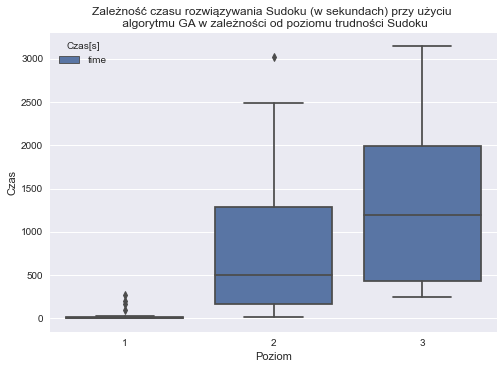
\includegraphics[width=0.5\columnwidth]{czas_poziom.png} % Example image
        \caption{Wykres pudełkowy zależności czasu rozwiązywania Sudoku przy użyciu Algorytmu Genetycznego dla plansz Sudoku o róznych trudnościach, gdzie 1 - oznacza poziom łatwy, 2 - poziom średni i 3 - poziom trudny. }
\end{figure}

Można na podstawie wykresu 5.6 zauważyć, że otrzymane wyniki zgadzają się z intuicją - dla plansz trudniejszych (będących większym problemem), Sudoku rozwiązywane jest znacznie dłużej.\\

\begin{figure}[h] % [h] forces the figure to be output where it is defined in the code (it suppresses floating)
        \centering
        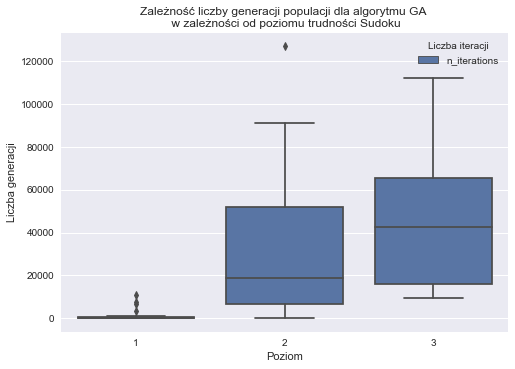
\includegraphics[width=0.5\columnwidth]{generacje_poziom.png} % Example image
        \caption{Wykres pudełkowy zależności liczby generacji wykonanych w celu rozwiązywania Sudoku przy użyciu Algorytmu Genetycznego dla plansz Sudoku o róznych trudnościach, gdzie 1 - oznacza poziom łatwy, 2 - poziom średni i 3 - poziom trudny. }
\end{figure}

Na podstawie wykresu 5.7 możemy zauważyć, że zależność liczby generacji w celu rozwiązania Sudoku do poziomu trudności jest odpowiednia zależności czasowej - fakt ten wynika z samej koncepcji Algorytmu Genetycznego - próby wykonywane były na tej samym rozmiarze populacji, stąd też liczba generacji jest odpowiednia do czasu.\\

\begin{figure}[h] % [h] forces the figure to be output where it is defined in the code (it suppresses floating)
        \centering
        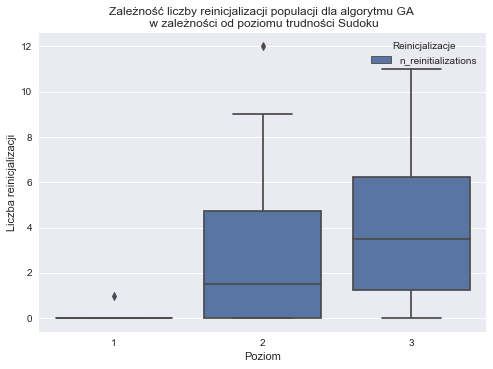
\includegraphics[width=0.5\columnwidth]{reinicjalizacje_poziom.png} % Example image
        \caption{Wykres pudełkowy zależności liczby reinicjalizacji kataklistycznych wykonanych w celu rozwiązywania Sudoku przy użyciu Algorytmu Genetycznego dla plansz Sudoku o róznych trudnościach, gdzie 1 - oznacza poziom łatwy, 2 - poziom średni i 3 - poziom trudny. }
\end{figure}

Wykresy 5.8 oraz 5.9 również są zgodne z intuicją - ze względu na stałość hiperparametrów, oczywistym jest, że liczba wywołań funkcji celu tak naprawdę jest liczbą generacji przemnożoną przez rozmiar populacji. W przypadku liczby dokonywanych reinicjalizacji (wykres 5.8) można zauważyć, że solver tylko raz potrzebował wykonywać reinicjalizację - świadczy o tym pojedynczy element odstający.\\ 

\begin{figure}[h] % [h] forces the figure to be output where it is defined in the code (it suppresses floating)
        \centering
        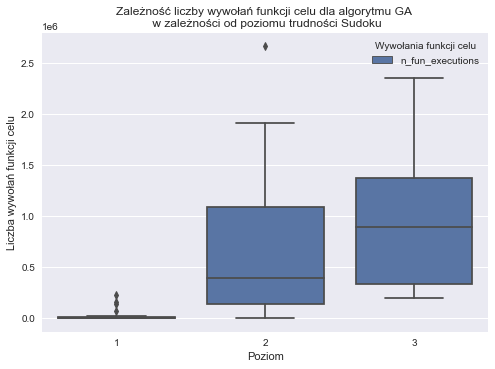
\includegraphics[width=0.5\columnwidth]{cel_poziom.png} % Example image
        \caption{Wykres pudełkowy zależności liczby wywołań funkcji dopasowania wykonanych w celu rozwiązywania Sudoku przy użyciu Algorytmu Genetycznego dla plansz Sudoku o róznych trudnościach, gdzie 1 - oznacza poziom łatwy, 2 - poziom średni i 3 - poziom trudny. }
\end{figure}

Na koniec zostało zamieszczone zestawienie tabelaryczne (tabele 5.2 i 5.3) poziomu trudności planszy Sudoku ze statystykami.\\

\begin{table}[h!]
\centering
\begin{tabular}{||c c c c c c c ||} 
 \hline
 Trudność & $\overline{T}$ [s] & $T_{min}$ [s] & $T_{max}$ [s] & $\overline{i}$ & $i_{min}$ & $i_{max}$ \\ [0.5ex] 
 \hline\hline
 łatwa  & 30.876 \pm 65.128 & 1.228 & 273.898 & 1221.7 \pm 2566.002 & 47 & 10757\\ 
 średnia & 898.3 \pm 1023.85 & 10.6 & 3020.753 & 35594.667 \pm 40799.175 & 365 & 126930\\ 
 ciężka  & 1284.8 \pm 972.874 & 247.744 & 3142.003 & 45555.9 \pm 33943.592 & 9633 & 111953\\ 
 [1ex] 
 \hline
\end{tabular}
\caption{Wyniki rozwiązywania - czas (T) i generacje (i) - plansz Sudoku przy użyciu Algorytmu Genetycznego dla plansz Sudoku o różnym poziomie.}
\label{table:1}
\end{table}

\\

\begin{table}[h!]
\centering
\begin{tabular}{||c c c c c c c ||} 
 \hline
 Trudność & $\overline{f}$ [s] & $f_{min}$ [s] & $f_{max}$ [s] & $\overline{r}$ & $r_{min}$ & $r_{max}$ \\ [0.5ex] 
 \hline\hline
 łatwa  & 25676.7 \pm 53886.046 & 1008 & 225918 & 0.033 \pm 0.183 & 0 & 1\\ 
 średnia &  747509 \pm 396249 & 7686 & 2665551 & 3.25 \pm 4.025 & 0 & 12\\ 
 ciężka  & 956694.9 \pm 891187.5 & 202314 & 2341034 & 4.1 \pm 3.542 & 0 & 11\\ 
 [1ex] 
 \hline
\end{tabular}
\caption{Wyniki rozwiązywania - liczba wywołań funkcji dopasowania (f) i liczba reinicjalizacji (r) - plansz Sudoku przy użyciu Algorytmu Genetycznego dla plansz Sudoku o różnym poziomie.}
\label{table:1}
\end{table}

Możemy zauważyć, że rozwiązania charakteryzuje duże odchylenie standardowe - wynika to z tego, że algorytm bazuje w dużym stopniu na losowości i istnieją próby odstające od reszty. Jedna z prób - dla planszy o poziomie średnim - spowodowała, że największa liczba generacji dla tych plansz była większa niż dla plansz trudnych.

\subsubsection{Zbadanie wpływu hiperparametrów}
\begin{figure}[h] % [h] forces the figure to be output where it is defined in the code (it suppresses floating)
        \centering
        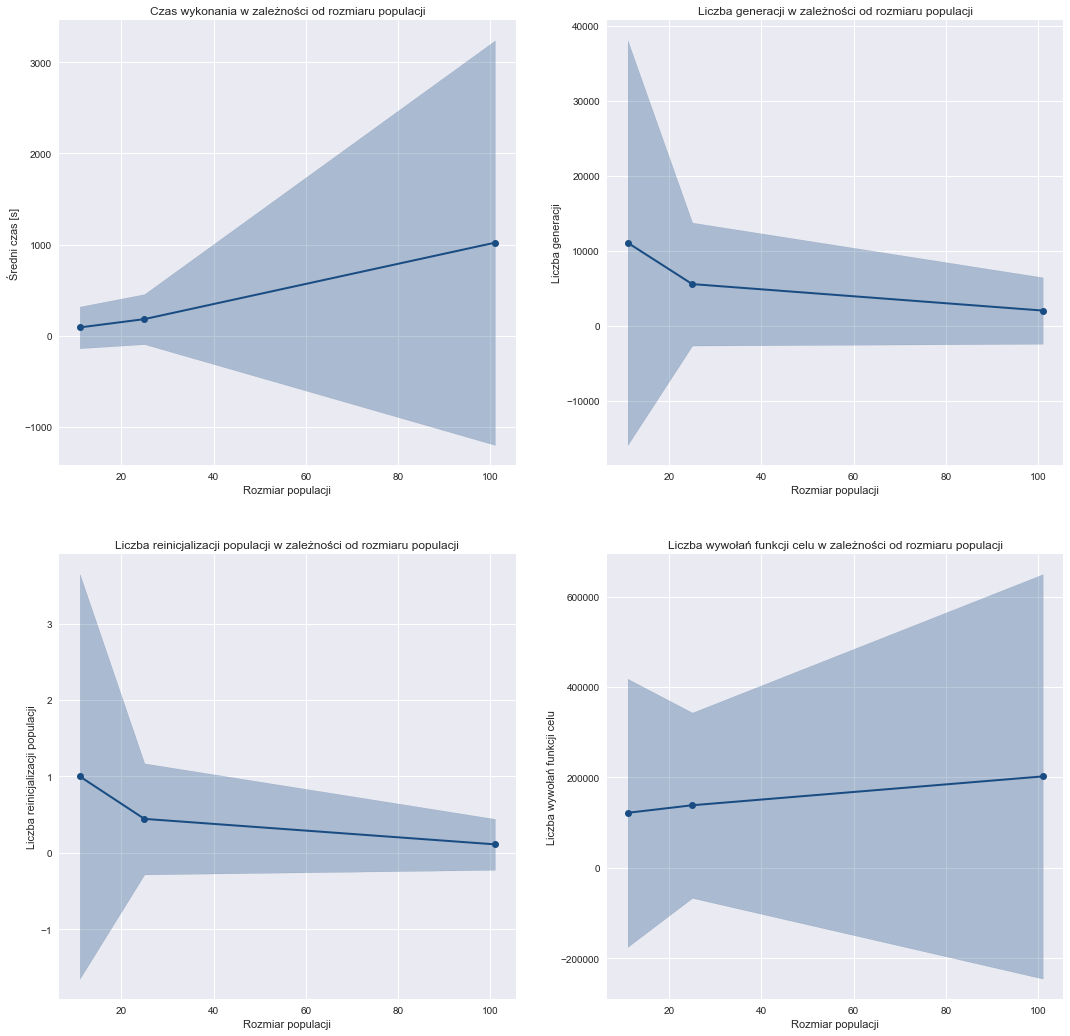
\includegraphics[width=0.8\columnwidth]{rozmiar_populacji.png} % Example image
        \caption{Wpływ rozmiaru populacji na efektywność algorytmu GA.}
\end{figure}\\


\\Następne przeprowadzone testy miały na celu zbadanie wpływu wartości hiperparametrów Algorytmu Genetycznego na jego efektywność. Testy zostały wykonane dla dwóch plansz o poziomie łatwym i jednej o poziomie średnim w postaci trzykrotnego uruchomienia algorytmu. Uśrednione wyniki każdego z testów przedstawiono na wykresach 5.10 - 5.13, odpowiednio dla następujących hiperparametrów:
\begin{itemize}
    \item wielkości populacji - wykres 5.10,
    \item prawdopodobieństwa mutacji - wykres 5.11,
    \item rozmiaru turnieju - wykres 5.12,
    \item prawdopodobieństwa krzyżowania - wykres 5.13.
\end{itemize}

Wykresy w górnym lewym rogu prezentują czas potrzebny do znalezienia rozwiązania, w górnym prawym rogu liczbę generacji, w dolnym lewym liczbę reinicjalizacji populacji, natomiast w dolnym prawym - liczbę wywołań funkcji dopasowania wykonanych przez solver Sudoku przy użyciu Algorytmu Genetycznego w zależności od wartości poszczególnych wartości hiperparametrów.\\

W przypadku tych testów, do algorytmu wprowadzony został dodatkowy parametr - jeśli rozwiązanie zajmowało będzie już 100000 generacji i wciąż nie znajdzie wyniku, wtedy uznane jest, że algorytm nie rozwiązuje danego Sudoku.\\


Na podstawie wykresu 5.10 można stwierdzić, że algorytm GA osiąga najlepsze wyniki dla mniejszej wielkości populacji. Im większa jest wielkość populacji, tym większy jest czas trwania rozwiązywania Sudoku oraz więcej razy wywoływana jest funkcja dopasowania. Na odwrót jest natomiast w przypadku liczby generacji populacji (iteracji algorytmu) i reinicjalizacji populacji - wynika to jednak z tego, że większa populacja oznacza więcej permutacji rozwiązania Sudoku w pojedynczej iteracji. Możemy więc tutaj zauważyć, że jeśli koszt wywołania funkcji celu nie jest zbyt duży, podejście z większym rozmiarem populacji może dać lepsze wyniki - w przypadku tego rozwiązania tak jednak nie było, stąd stosowanie mniejszej populacji okazało się bardziej efektywne.\\
\begin{figure}[h] % [h] forces the figure to be output where it is defined in the code (it suppresses floating)
        \centering
        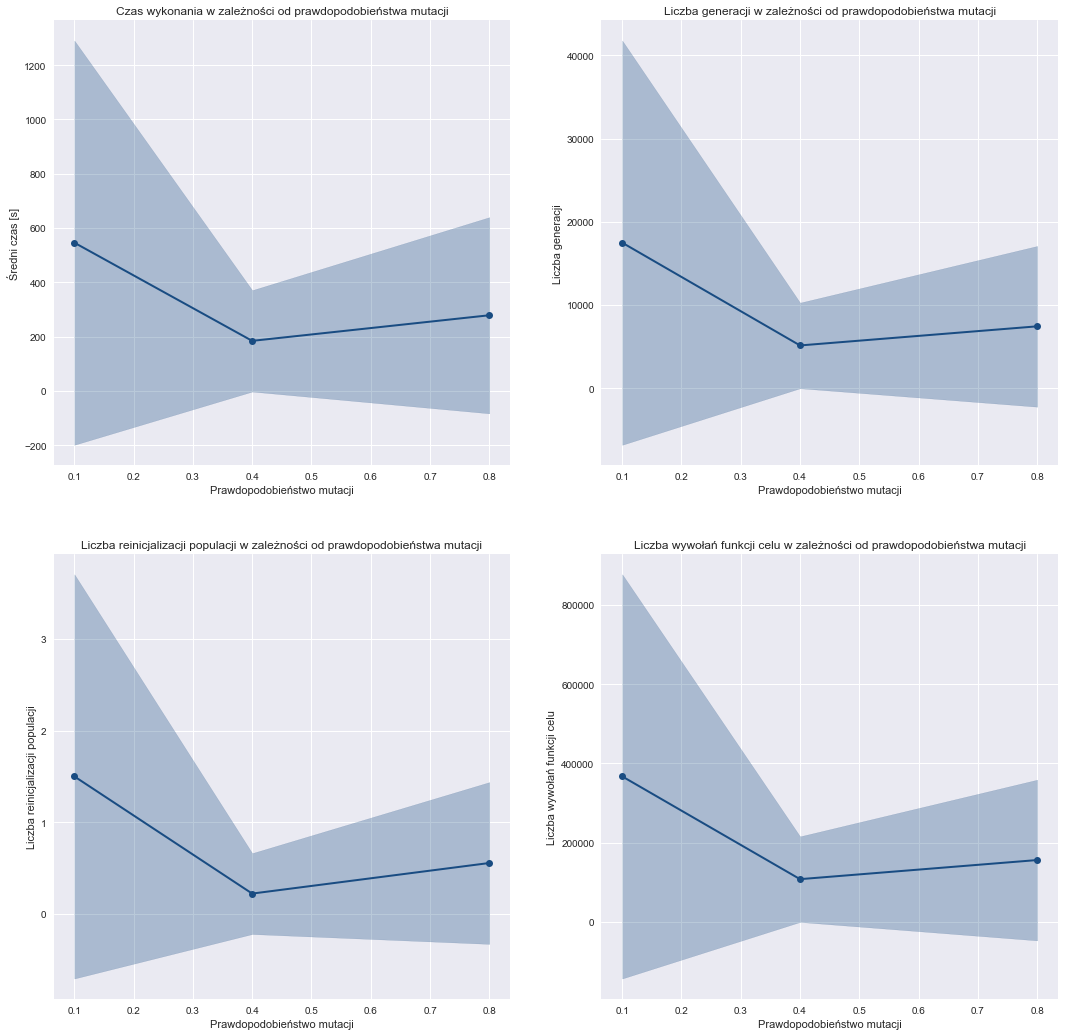
\includegraphics[width=0.8\columnwidth]{pstwo_mutacji.png} % Example image
        \caption{Wpływ prawdopodobieństwa mutacji na efektywność algorytmu GA.}
\end{figure}

Na podstawie wykresu 5.11 można zauważyć, że wybór prawdopodobieństwa mutacji może mieć znaczący wpływ na działanie algorytmu - zauważmy, że w przypadku wybrania bardzo małej wartości prawdopodobieństwa mutacji (rzędu 0.1), każda z miar efektywności daje najgorsze wyniki - wiąże się to z charakterystyką problemu Sudoku - jest to problem posiadający wiele optimów lokalnych, a małe prawdopodobieństwo mutacji oznacza bardzo dużą eksploatację - algorytm będzie reinicjalizował populację do momentu, aż wylosowana zostanie populacja startowa zbliżająca do optimum globalnego. W przypadku tego prawdopodobieństwa doszło również do jeszcze jednego problemu - jest to jedyny przypadek, gdy algorytm nie znalazł rozwiązania w 10000 generacjach. \\
W przypadku zbyt dużego prawdopodobieństwa mutacji również możemy zauważyć, że wszystkie z miar jakości się pogarszają, ale nie tak znacząco jak w przypadku małego prawdopodobieństwa - widzimy więc, że dużo korzystniejsze wydaje się postawienie na eksplorację, niż eksploatację w przypadku tego problemu.\\

\begin{figure}[h] % [h] forces the figure to be output where it is defined in the code (it suppresses floating)
        \centering
        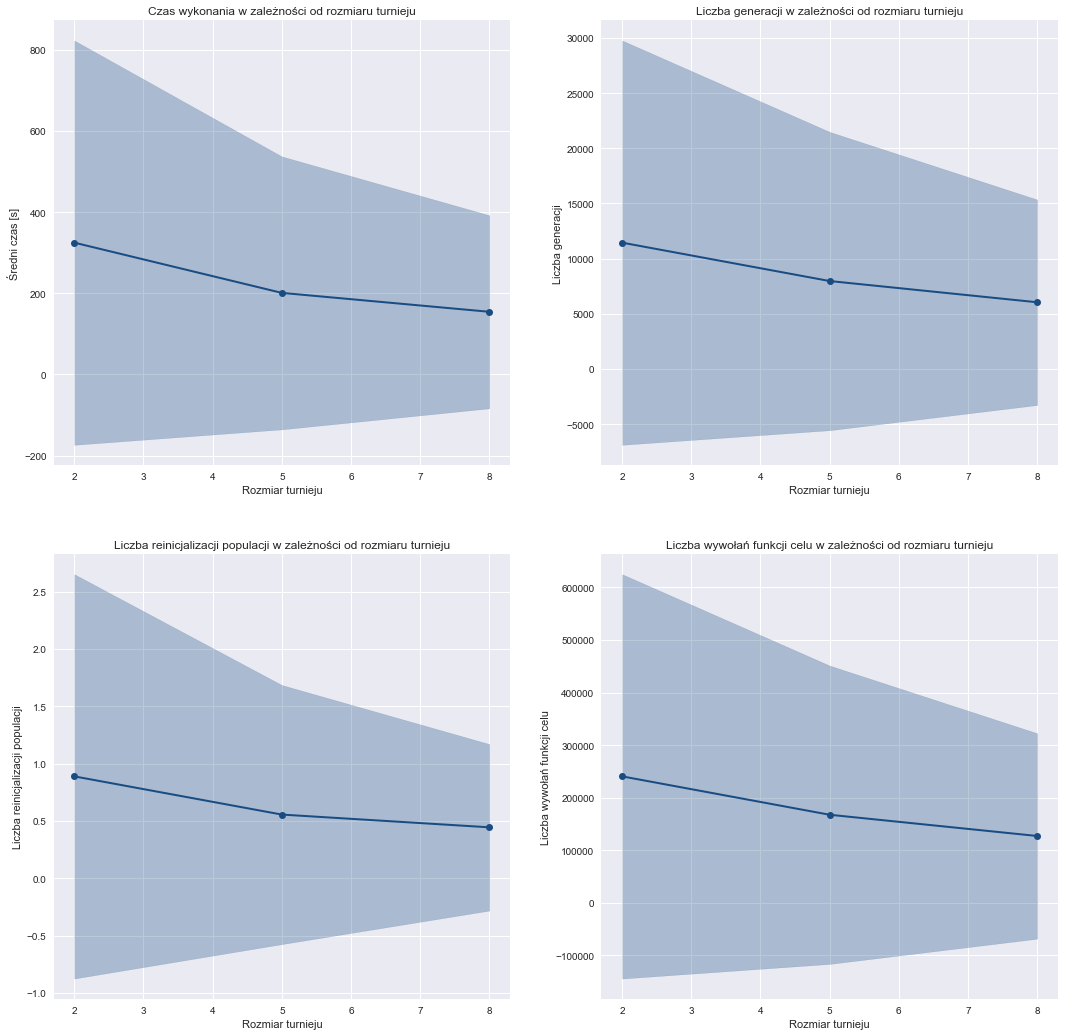
\includegraphics[width=0.8\columnwidth]{rozmiar_turnieju.png} % Example image
        \caption{Wpływ rozmiaru turnieju na efektywność algorytmu GA.}
\end{figure}

Na podstawie wykresu 5.12 można stwierdzić, że algorytm GA osiąga lepsze wyniki dla większego rozmiaru turnieju - wynika to z faktu, że dla bardzo małego rozmiaru turnieju, do krzyżowania trafiają gorsze osobniki z populacji - na nich krzyżowanie nie daje najlepszych efektów, stąd też takie wyniki. 
\\
Dobrym pomysłem w przypadku tego badania, byłoby sprawdzenie zachowania algorytmu przy zbadaniu jego działania, gdy mamy rozmiar turnieju bliski rozmiaru populacji - możemy się jednak domyślić, że wtedy ogromna skłonność do eksploatacji (ciągłe wybieranie najlepszych osobników z populacji i ich krzyżowanie) by negatywnie wpłynęła na działanie algorytmu - analogicznie jak w przypadku prawdopodobieństwa mutacji.\\

\begin{figure}[h] % [h] forces the figure to be output where it is defined in the code (it suppresses floating)
        \centering
        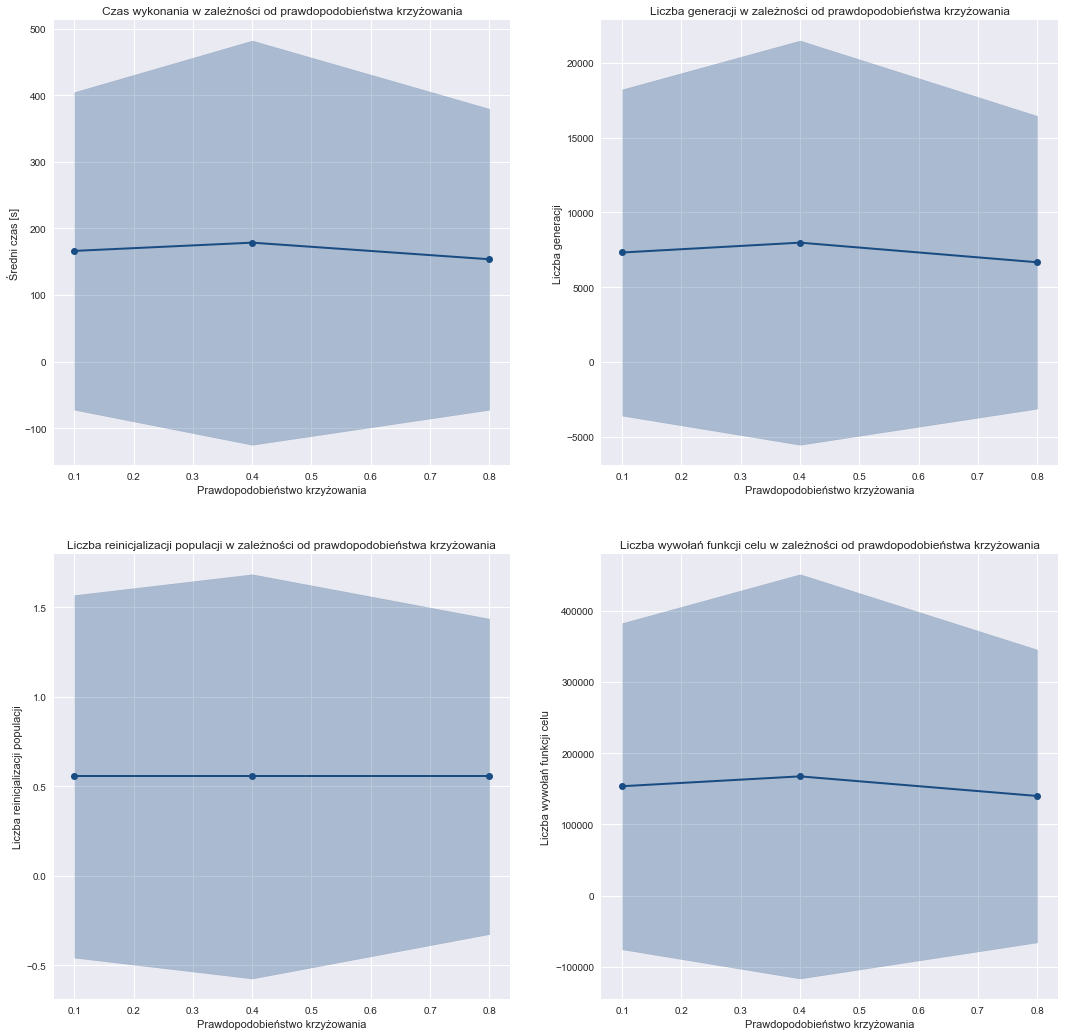
\includegraphics[width=0.8\columnwidth]{pstwo_krzyzowania.png} % Example image
        \caption{Wpływ prawdopodobieństwa krzyżowania na efektywność algorytmu GA.}
\end{figure}

Na podstawie wykresu 5.13 można stwierdzić, że wpływ prawdopodobieństwa krzyżowania na efekty działania algorytmu GA jest bardzo mały w porównaniu do innych hiperparametrów - zależność jest prawie linią poziomą.\\  

\subsection{Porównanie efektywności algorytmów}

\begin{table}[h!]
\centering
\begin{tabular}{||c c c c c c ||} 
 \hline
 Algorytm & Trudność & Nazwa & $\overline{T}$ [s] & $T_{min}$ [s] & $T_{max}$ [s]\\ [0.5ex] 
 \hline\hline
 GA & ciężka & board2 & 1284.798 \pm 922.863 & 247.743 & 3142\\ 
 ACO & ciężka & board2 & 0.008 \pm 0 & 0.007 & 0.009 \\
 GA & średnia & board1 & 564.808 \pm 357.184 & 202.609 & 1081.03 \\ 
 ACO & średnia & board1 & 0.007 \pm 0 & 0.007 & 0.008 \\ 
  GA & średnia & board2 & 2023.042 \pm 860.452 & 705.906 & 3020.752 \\ 
 ACO & średnia & board2 & 0.007 \pm 0 & 0.007 & 0.008 \\ 
  GA & średnia & board3 & 107.051 \pm 111.566 & 10.604 & 296.358 \\ 
 ACO & średnia & board3 & 0.009 \pm 0.006 & 0.007 & 0.029 \\
  GA & łatwa & board1 & 34.397 \pm 80.131 & 1.265 & 273.898 \\ 
 ACO & łatwa & board1 & 0.007 \pm 0 & 0.007 & 0.008 \\ 
  GA & łatwa & board2 & 51.63 \pm 69.501 & 1.698 & 194.681 \\ 
 ACO & łatwa & board2 & 0.007 \pm 0 & 0.007 & 0.008 \\ 
  GA & łatwa & board3 & 6.598 \pm 4.101 & 1.228 & 13.829 \\ 
 ACO & łatwa & board3 & 0.009 \pm 0.006 & 0.007 & 0.029 \\ [1ex] 
 \hline
\end{tabular}
\caption{Porównanie czasów znalezienia rozwiązań dla tych samych plansz.}
\label{table:1}
\end{table}

Na podstawie analizy czasów potrzebnych na znalezienie rozwiązania przez oba algorytmy dla tych samych plansz zauważyć można bardzo dużą różnicę w efektywności algorytmów dla zadania rozwiązywania Sudoku. Porównania zostały przeprowadzone dla plansz, w których algorytm genetyczny był w stanie znaleźć rozwiązanie w rozsądnym i dopuszczalnym czasie. Algorytm ACO bardzo szybko znalazł rozwiązania dla wszystkich tych plansz. Czasy dla algorytmu genetycznego są o rzędy wielkości większe. \\

Analizując nasze wyniki można dojść do wniosku, że algorytm genetyczny słabo sprawdza się w zadaniu rozwiązywania Sudoku. Algorytm ACO natomiast odniósł świetne wyniki i jego zastosowanie do badanego problemu znajduje bardzo zasadne zastosowanie.

\section{Bibliografia}
[1] Mirjalili, S. (2019). "Evolutionary Algorithms and Neural Networks: Theory and Applications". Griffith University Brisbane, QLD: Springer International Publishing.

[2] Lloyd, H. and Amos, M. (2020). "Solving Sudoku With Ant Colony Optimization". IEEE.

[3] Dorigo, M., Birattari, M. and Stutzle, T. “Ant Colony Optimization” J. Autom., IEEE, 2006.

[4] T. Mantere and J. Koljonen, "Solving, rating and generating Sudoku puzzles with GA," 2007 IEEE Congress on Evolutionary Computation, 2007, pp. 1382-1389, doi: 10.1109/CEC.2007.4424632.

\end{document}
